\chapter{Tests}\label{ch:tests}
Med koden designet og implementeret, kan tests af koden påbegyndes. Tests er en del af Unified Process modellen\cite{UnifiedProcess}, hvori den fremgår både under Inception og Elaboration fasen (det gælder også Construction og Transistion, men det ikke relevant for dette projekt). Tests er en nødvendig del af Unified Process, ikke fordi det program der bliver lavet ikke må have nogle fejl, men fordi det kan give et godt overblik over hvad der kan forbedres\cite{sestoft2008systematic}. Der er brugt JUnit 5\cite{JUnit} til at teste de forskellige metoder. Herunder ses det også, at White-Box testing, samt Black-box testing benyttes. 

\section{Fremgangsmåde}
White-box testing er at teste funktionaliteten af selve programmet. Altså, at alle delene internt i programmet er blevet udført. Under White-box testing laves der en test-miljø, og ud fra bestemte inputs undersøges det om de forventede outputs kommer tilbage. Det gode ved White-box testing er, at det både er en god systematisk metode til at opdage fejl, og viser samtidig alle dele af programmet virker. Måden det foregår på, er at for hver eneste data input sæt der bruges, skal der også være et forventet output specificeret. Herefter vil programmet køre med alle data input-sæt og de givende outputs bliver sammenlignet med de forventede\cite{sestoft2008systematic}.

Black-Box testing skal sørge for at programmet løser det cetrale problem den er sat til at løse. Her laves igen et test-datasæt med inputs og forventede outputs, men her omhandler det mere om problemet kan løses for almindelige og ekstreme inputs. Derfor vil det være en god ide, hvis testeren på forhånd har en idé om hvilke problemer der skal testes, for at kunne få programmet til at løse det\cite{sestoft2008systematic}. 

Vores tests bliver primært unit-tests, der er implementeret efter AAA-mønstret (Arrange, Act, Assert), hvor tests bliver eksekveret i tre skridt\cite{ArrangeActAssert}:
\begin{description}
    \item[Arrange:] præ-konditioner for testen sættes op.
    \item[Act:] metoder, der testes på, bliver eksekveret
    \item[Assert:] forventede udfald bliver sammenlignet med faktiske udfald 
\end{description}

\section{Implementering af tests}
Vi gør brug af følgende biblioteker til at køre vores tests:
\begin{itemize}
    \item JUnit 5.4
    \item Mockito 3.3.3
\end{itemize}

\subsection{JUnit}
JUnit\cite{JUnit} er et Java testing framework, der bruges til at definere test-klasser med tilhørende test-metoder. Disse test-metoder instantierer og kalder metoder i en klasse i programmet, kaldet SUT eller "System Under Test". En test-klasse, der gør brug af JUnit, vil typisk følge en struktur lignende eksemplet i Listing~\ref{lst:JUnitEksempel}

I dette eksempel bliver følgende annotationer brugt\cite{JUnitDocumentation}: 
\begin{description}
    \item[\texttt{@BeforeAll}:] Denne metode bliver kaldt før alt andet i klassen.
    \item[\texttt{@BeforeEach}:] Denne metode bliver kaldt før hver enkelt test.
    \item[\texttt{@Test}:] Test-metode.
    \item[\texttt{@AfterEach}:] Bliver kaldt efter hver test.
    \item[\texttt{@AfterAll}:] Bliver kaldt til allersidst.      
\end{description}

Yderligere gøres der brug af JUnit's assert-metoder. En assert-metode definerer et forventet udfald af en test. Der findes adskillige assert-metoder i JUnit, der definerer forskellige former for forventede udfald, herunder \texttt{assertEquals}, \texttt{assertTrue}/\texttt{assertFalse}, og \texttt{assertArrayEquals} som sammenligner variabler med deres forventede værdier. Yderligere findes \texttt{assertNull}/\texttt{assertNotNull}, som tester om en givet reference er null. Til sidst findes \texttt{assertAll} og \texttt{assertThrows}, som bruges til at teste, at givne funktionskald henholdsvis eksekveres uden fejl og kaster en undtagelse\cite{JUnitDocumentation}.

Vi gør brug af JUnit 5.4 grundet kompabilitet med mocking-biblioteket Mockito.

\begin{listing}
    \inputminted[
        frame=lines,
        framesep=2mm,
        baselinestretch=1.2,
        bgcolor=LightGray,
        fontsize=\footnotesize,
        linenos
    ]{java}{listings/junitExample.java}
    \caption{Exempel på en JUnit test-klasse\label{lst:JUnitEksempel}}
\end{listing}

\subsection{Mockito}
Mockito \cite{Mockito} er et mocking-bibliotek, der bruges i samspil med JUnit. Det tillader os at "mocke", det vil sige, lave stedfortræder-klasser i vores tests. Det har det formål, at vi kan isolere vores SUT fra dets dependencies, så vi kan udføre unit-tests på de metoder, der gør brug af disse dependencies. Dette er specielt brugbart når vi tester vores controller-klasser.

I Listing~\ref{lst:MockEkempel} ses det hvordan mocks bliver defineret som felter i en test-klasse. \texttt{@Mock}-annotationen signalerer, at det er en stedfortræder-klasse. \texttt{@InjectMocks} signalerer, at stedfortræderne skal indsættes i denne klasse.

I Listing~\ref{lst:MockTestEksempel} ses et eksempel på en test-metode, der gør brug af mocks. Nøgleordene \texttt{when} og \texttt{verify} er statiske metoder i Mockito-biblioteket. I eksemplet bruges \texttt{when} sådan, at når \texttt{myMethod} is \texttt{MyClass1} bliver kaldt, så skal den returnere '1' \textit{i stedet for} at kalde den reelle metode. 

\begin{listing}
    \begin{minted}
    [
        frame=lines,
        framesep=2mm,
        baselinestretch=1.2,
        bgcolor=LightGray,
        fontsize=\footnotesize,
        linenos
    ]{java}
@Mock private MyClass1 myMockedClass1;
@Mock private MyClass2 myMockedClass2;
@InjectMocks private ClassUnderTest classUnderTest;
    \end{minted}
    \caption{Eksempel på brug af mocks \label{lst:MockEkempel}}
\end{listing}

\begin{listing}
    \begin{minted}
    [
        frame=lines,
        framesep=2mm,
        baselinestretch=1.2,
        bgcolor=LightGray,
        fontsize=\footnotesize,
        linenos
    ]{java}
@Test
public void testMethod() {
        when(myMockedClass1.myMethod()).thenReturn(1);
        classUnderTest.methodUnderTest();
        verify(myMockedClass1, times(1)).myMethod();
        verify(myMockedClass2, never()).otherMethod();
}
    \end{minted}
    \caption{Eksempel på brug af mocks i en test-metode\label{lst:MockTestEksempel}}
\end{listing}

\texttt{verify} fungerer som en assertion: den tester i bund og grund, om en givet metode bliver kaldt, hvor mange gange den bliver kaldt, og hvilke argumenter den bliver kaldt med. I eksemplet bliver det først asserted, at \texttt{myMethod} i \texttt{MyClass1} bliver kaldt én gang med en tom parameterliste. Dernæst bliver det asserted, at \texttt{otherMethod} i \texttt{MyClass2} aldrig bliver kaldt. Dermed kan vi teste på, hvilke beskeder bliver sendt til andre klasser.

\section{Test cases}
For at gå systematisk til værks, skal der opsættes et skema med test cases\cite{Heumann}. Der bliver altså lavet flere scenarier som først blive sat op i skemaet, så testet i programmet, og til sidst vil der foretages ændringer i koden, som kan fikse de opståede problemer, hvorefter de samme tests køres igen. Tests er foretaget på version: 57a8dfa af programmet, og vores test cases kan ses i Bilag~\ref{app:testcases}.

\subsection{Unit tests}
\subsubsection{Regression Tests}
\todo{insert unit test skema}
Test-klassen \texttt{RegressionTest} tester vores regressions algoritme, og for at teste dette skal der bruges en massiv mængde data. Derfor bruges en csv-fil, som beskriver relationerne mellem forskellige typer cement, og denne csv-fil kan findes på \texttt{res/concrete.csv}, og selve test koden kan findes på \texttt{src/hjem/is/test/RegressionTest.java}. \texttt{concrete.csv} består af test data hentet online~\cite{ExampleSales}. I disse tests bruges en assert metode, som vi selv har lavet, kaldet \texttt{assertApproxEquals}. Denne bruges eftersom at regression ikke handler om at lave et 100\% perfekt estimat, men bare godt nok til at det er brugbart.

Ved udførsel af testen hentes concrete.csv filen ind i en \texttt{@BeforeAll}, eftersom at alle test bruger den samme data. Data'en laves om til \texttt{Observation} objekter, eftersom at det er den type objekt vores implementation bruger som argument. Begge tests tester at algoritmen kan forudsige at \texttt{compressivestrength} på index 30 passer med index for en delta (forskel)på 20 af den faktiske værdi, begge tests printer også deres $r^{2}$ værdi og deres præcision.

Den første test tester \texttt{GradientDescentFit}\cite{GradientDescent} implementation, hvor der bruges en alpha af 0.0001, den anden tester \texttt{NormalEquationFit}\cite{NormalEquation}. Begge tests består her. 

\subsubsection{Controller tests}
\texttt{StoragePlanControllerTest} og \texttt{PeriodicPlanControllerTest} er unit test-klasser for henholdsvis \texttt{StoragePlanController} og \texttt{PeriodicPlanController}. Disse tests er lavet ud fra vores test cases - vi har kigget på hver enkelt test case og vurderet, hvad den enkelte controller-klasses ansvar er i et givet scenarie, og så har vi skrevet en test, der tester for dét.

\subsection{Integration tests}
Integration tests er tests som beskriver og tester, hvordan lagene i programmet interager med hinanden. Et godt eksempel er test af DAO \cite{DAO}, eftersom både metoden på DA objektet, og dens interaktion med databasen bliver testest i disse test cases.
\todo{write stuff here about our integration tests}
%most important tests
%What it tests
%how it works
%did it pass?

\subsection{System tests}
For at gå endnu et niveau op, blev der også lavet system tests\cite{TestLevels}. Under system testing afprøves forskellige flows af den centrale use case, i dette tilfælde vores tages der udgangspunkt i Fully Dressed Use Case fra kapitel \ref{fullydressed}.

Under figur \ref{fig:testgenerate} ses første iteration af test af UI. Herunder blev det testet, om det var muligt for en lagerplan at blive oprettet. Det viser sig, at det er muligt at oprette lagerplanen med både forskellige navne og tal. Dog bliver den gemte lagerplan ikke vist. Stadig en succes, eftersom målet var at få lagerplanen gemt, herefter kan det implementeres, at den gemte lagerplan også bliver vist frem i UI. På den anden side blev test case nr. 4 ikke en succes, da den gemte navnet "navn", hvilket ikke skulle være meningen. I stedet skulle den foreslå at man foretager en navneændring.

\begin{figure}[p]
    \centering
    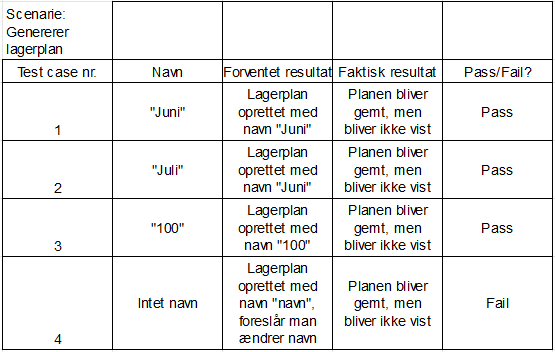
\includegraphics[width=0.7\hsize]{figures/tests/test_generer_plan.png}
    \caption{Scenarie: En lagerplan skal genereres}
    \label{fig:testgenerate}
\end{figure}

Det skulle herunder gerne være muligt, at rette en eksisterende lagerplan. Testskemaet på figur \ref{fig:testedit} tester, at når man er inde på lagerplanen, skulle det være muligt at redigere mængden af varer, om planen er aktiv eller ej, og at se hvilken periode man redigerer. Dette var dog ikke muligt at gøre, eftersom display af lagerplanen ikke eksisterer. Ud fra testen bliver der evalueret og derefter skal det implementeres således, at det er muligt at klikke ind på en lagerplan og rette den. 

\begin{figure}[p]
    \centering
    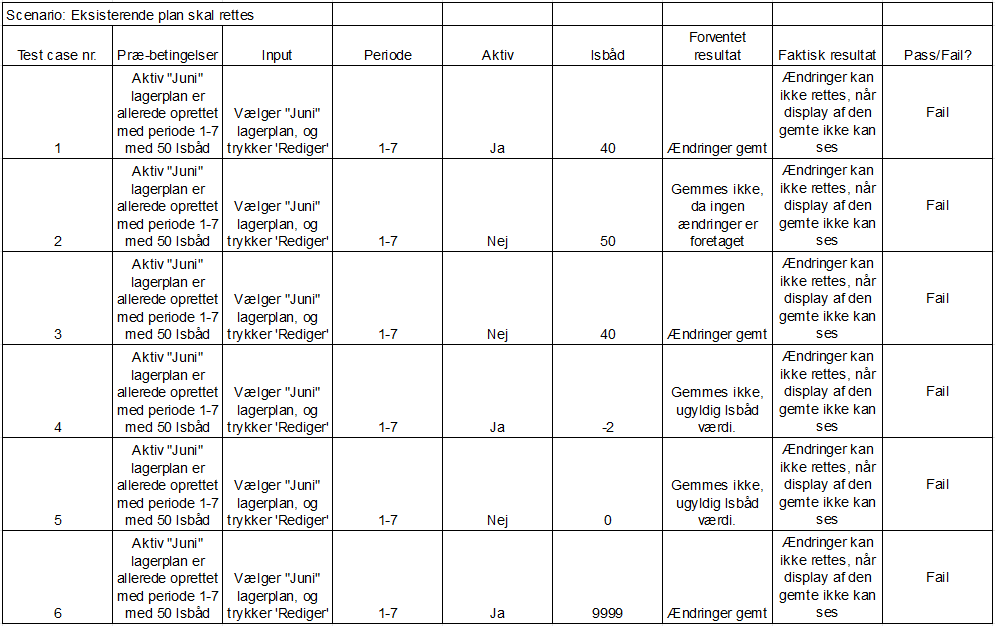
\includegraphics[width=0.7\hsize]{figures/tests/edit_existing_plan.png}
    \caption{Scenarie: En lagerplan skal rettes}
    \label{fig:testedit}
\end{figure}

Det skulle være muligt at generere en plan, rette i planen ved f.eks. at tilføje et produkt, og så gemme planen igen. Ud fra testskemaet på figur \ref{fig:testeditperiod} kan det ses, at til trods for at gem-metoderne er testet, så fungerede det ikke samme med UI på dette tidspunkt. Det skal evalueres sådan at det kan virke ordenligt.

\begin{figure}[p]
    \centering
    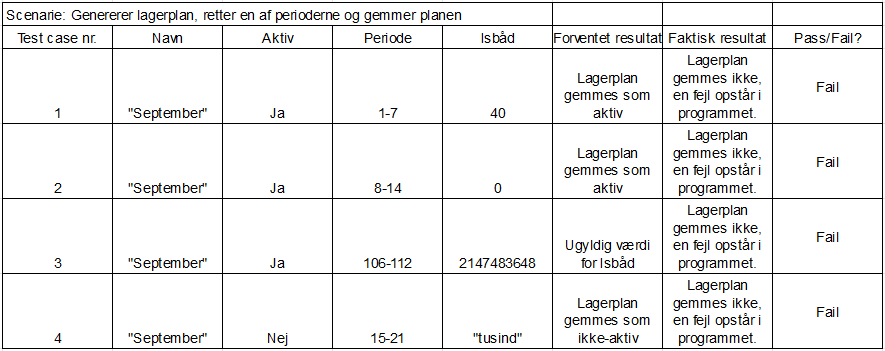
\includegraphics[width=0.7\hsize]{figures/tests/test_ret_plan.png}
    \caption{Scenarie: En periode i lagerplanen rettes}
    \label{fig:testeditperiod}
\end{figure}

Det skulle være muligt at slette en lagerplan, som allerede er oprettet. Som testskemaet på figur \ref{fig:testdelete} viser, så var det på det tidspunkt ikke muligt at vise planerne, så man kunne tilgå "slet" knappen. Derfor fejler begge tests. For at løse det skulle planerne selvfølgelig vises, sådan at det er muligt at rette og slette dem. UI for lagerplanen var ellers implementeret og virkede, men under testen her fejlede det.

\begin{figure}[h]
    \centering
    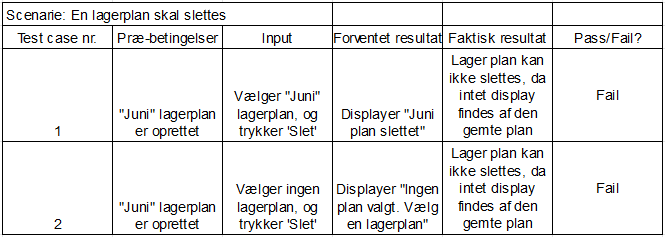
\includegraphics[width=0.7\hsize]{figures/tests/test_slet_lagerplan.png}
    \caption{Scenarie: En lagerplan skal slettes}
    \label{fig:testdelete}
\end{figure}





